\documentclass{VUMIFPSbakalaurinis}
\usepackage{algorithmicx}
\usepackage{algorithm}
\usepackage{algpseudocode}
\usepackage{amsfonts}
\usepackage{amsmath}
\usepackage{bm}
\usepackage{caption}
\usepackage{color}
\usepackage{float}
\usepackage{graphicx}
\usepackage{listings}
\usepackage{subfig}
\usepackage{wrapfig}
\usepackage{tabularx}

\usepackage{enumitem}
%PAKEISTA, tarpai tarp sąrašo elementų
\setitemize{noitemsep,parsep=0.7pt,partopsep=0.7pt}
\setenumerate{noitemsep,parsep=0.7pt,partopsep=0.7pt}

% Titulinio aprašas
\university{Vilniaus universitetas}
\faculty{Matematikos ir informatikos fakultetas}
\department{Programų sistemų katedra}
\papertype{Bakalauro darbas}
\title{Programų sistemų kūrimo metodų tyrimas}
\titleineng{Investigation Methods of Software Development}
\author{Vardenis Pavardenis}
% \secondauthor{Vardonis Pavardonis}   % Pridėti antrą autorių
\supervisor{prof. habil. dr. Vardaitis Pavardaitis}
\reviewer{doc. dr. Vardauskas Pavardauskas}
\date{Vilnius – \the\year}

% Nustatymai
% \setmainfont{Palemonas}   % Pakeisti teksto šriftą į Palemonas (turi būti įdiegtas sistemoje)
\bibliography{Bakalaurinis}

\begin{document}
\maketitle

%% Padėkų skyrius
% \sectionnonumnocontent{}
% \vspace{7cm}
% \begin{center}
%     Padėkos asmenims ir/ar organizacijoms
% \end{center}

\sectionnonumnocontent{Santrauka}

Šiame darbe nagrinėtas blokų grandinės technologijos tinkamumas skaitmeninės tapatybės valdyme. Pristačius naudotojų poreikius identiteto valdymui internete,
apžvelgtas esamų modelių gebėjimas juos išpildyti. Apibendrinus liekančias naudotojų problemas, tirta blokų grandinė ir jos charakteristikos,
kurios leistų įveikti kylančius iššūkius skaitmeninės tapatybės valdyme.

Nustatyta, kad blokų grandinė gali būti taikoma skaitmeninės tapatybės valdymui internete. Pristatytas blokų grandine ir išmaniaisias kontraktais
paremtas atributų valdymo modelis,
leidžiantis naudotojams kontroliuoti savo asmens duomenis ir jų sklaidą. Sukurtas pateikto modelio prototipas, parašytas su \enquote{Solidity}
programavimo kalba.

\raktiniaizodziai{skaitmeninė tapatybė, skaitmeninės tapatybės valdymas, blokų grandinė, išmanieji kontraktai.}   

% English version

\sectionnonumnocontent{Summary}
In this paper, blockchain applicability for digital identity management was investigated. After presenting user needs for identity management,
currently used identity management models were researched. Following that, blockchain and its characteristics were examined,
in order to find out whether the technology is suitable
to overcome present user identification challenges.

It was determined that blockchain can be used for digital identity management in the internet. A blockchain and smart contract based attribute management model was presented,
which allows users to take control of their own personal data and it's distribution. A prototype of the model was presented,
which was written in \enquote{Solidity} programming language.

\keywords{digital identity, digital identity management, blockchain, smart contracts.}

\sectionnonum{Įvadas}
Interneto paslaugos šiais laikais yra neatsiejama žmonių gyvenimo dalis.
Norėdami individualizuoti turinį, sustiprinti taikomosios programos saugumą ar siekdami
iš anksto išvengti kenkėjiškų tikslų turinčių asmenų ar sukurtų robotų, paslaugų tiekėjai
siekia identifikuoti savo naudotojus. Interneto naudotojų skaičiui perkopus 4 milijardus \cite{InternetUsers2018},
o kiekvienam naudotojui vidutiniškai turint po 7 skirtingas socialines paskyras \cite{Mander2017}, asmenų
tapatybių valdymas, autentifikavimas ir autorizavimas tampa vis didesniu iššūkiu.

Tapatybių valdymas kelia problemų tiek paslaugų tiekėjams, tiek jų naudotojams. Kiekvienas
paslaugų tiekėjas turi skirti papildomų resursų naudotojų tapatybių valdymui, jų autentifikavimui,
jautrių duomenų saugumo užtikrinimui. Paslaugų naudotojams bene didžiausi atsiradę keblumai:
milžiniškas įsimintinų slaptažodžių kiekis bei sunkumai kontroliuojant savo asmens duomenų sklaidą
skirtingose sistemose. Vidutiniškai interneto naudotojas turi 25 slaptažodžių reikalaujančias paskyras
ir per dieną turi įvesti 8-is slaptažodžius \cite{Florencio2007}. Susidarius tokiai situacijai, per didelis įsimintinų slaptažodžių kiekis neretai 
priverčia naudotojus paaukoti saugumą dėl patogumo
ir pradėti naudoti tą patį slaptažodį sirtingoms sistemoms \cite{Pashalidis2003, Samar1999}. Naudotojas, turėdamas keletą
paskyrų skirtingose sistemose, taip pat praranda dalį savo asmens duomenų kontrolės. Jam tenka pasitikėti
taikomosios programos naudojamomis technologijomis ir metodais ir tikėtis, kad jie bus pakankamai saugūs
ir stabilūs bei suteikti asmens duomenys nepasieks nepageidaujamų adresatų. Didėjant naudojamų paslaugų kiekiui,
naudotojo skaitmeninės tapatybės duomenis turi vis daugiau taikomųjų programų ir bent vienai iš jų
patyrus programišių įsilaužimą ar kitokią nesėkmę, jautrūs naudotojo duomenys būna paviešinti. 

Vienu iš pagrindinių skaitmeninės tapatybės valdymo keliamų problemų sprendimu išlieka vienkartinis prisijungimas
 (angl. \textit{Single Sign-On}). Šis sprendimas leidžia naudotojui pasirinkti
vieną tapatybės tiekėją (angl. \textit{identity provider}) ir patikėti jam skaitmeninės tapatybės valdymą. Tuomet naudotojas prie visų
paslaugų, palaikančių pasirinkto tapatybės tiekėjo (pvz. \textit{Facebook}) prisijungimą, gali autentifikuotis naudodamas ta pačia paskyra. Tokiu
būdu naudotojui pakanka prisiminti tik slaptažodžius, užregistruotus tapatybės tiekėjų sistemose, o paslaugų
tiekėjai neturi patys rūpintis autentifikavimu ar autorizavimu, o jį užtikrina integruodami sistemą
su tapatybės tiekėju. Tačiau šis sprendimo būdas taip pat turi aiškių trūkumų: naudotojas negali prisijungti
prie paslaugų, nepalaikančių pasirinkto tapatybės tiekėjo, dėl paslaugų tiekėjų priklausomybės nuo tapatybės tiekėjo pastarojo pasiekiamumas
tampa vieninteliu nesėkmės tašku (angl. \textit{single point of failure}), naudotojas taip pat praranda dalį savo asmens duomenų kontrolės.
Naršantis internete asmuo yra priverstas pasitikėti tapatybės tiekėjo
gebėjimu perduoti tik naudotojo leistus asmens duomenis ir tik toms trečiosioms šalims, kurias jis patvirtina.
Kaip rodo \textit{Cambridge Analytica} incidentas \cite{CambridgeAnalytica}, net didžiosios kompanijos, tokios
kaip \textit{Facebook}, ne visada sugeba tai užtikrinti.

Blokų grandinė (angl. \textit{blockchain}) yra nauja alternatyva skaitmeninės tapatybės valdymui. Ši technologija veikia kaip
paskirstytų įrašų platforma (angl. \textit{distributed ledger platform}), kurioje kiekvienas įrašas yra nekintamas (angl. \textit{immutable}), o visi
užfiksuoti įrašai atspindi tikslią transakcijų istoriją nuo pat grandinės sukūrimo \cite{Baars2016}. Saugant tapatybės duomenis šioje grandinėje ir
pritaikius reikiamą blokų grandinės pasiekiamumo lygį įrašų rašymui ir skaitymui, asmuo visada
žino, kokia trečioji šalis gali pasiekti kokius tapatybės duomenis. Kadangi blokų grandinė yra decentralizuota, pritaikius ją skaitmeninių tapatybių valdyme taip pat
būtų galima išvengti šioje srityje dažnos vienintelio nesėkmės taško problemos. Šiame darbe nagrinėjama, kada verta naudoti blokų grandinę
naudotojų skaitmeniniam autentifikavimui bei autorizavimui, kokie to pranašumai, trūkumai bei priėmimo barjerai (angl. \textit{adoption barriers}).
\\

\textbf{Darbo tikslas} - išanalizuoti blokų grandinės tinkamumą skaitmeninės tapatybės valdymui.
\\

\textbf{Darbe keliami uždaviniai}:

\begin{enumerate}
    \item Išnagrinėti esamus skaitmeninės tapatybės valdymo sprendimus ir jų keliamus iššūkius.
    \item Apibūdinti blokų grandines ir jų savybes, leidžiančias spręsti dabartines identifikavimo problemas.
    \item \textit{Apžvelgti esamas blokų grandinės sistemas, taikomas naudotojų autentifikavimui ar autorizavimui}.
    \item Pateikti blokų grandinės panaudos atvejį skaitmeninės tapatybės valdymui ir sukurti jo veikimą demonstruojantį prototipą.
    \item Įvertinti pateikto sprendimo tinkamumą apibūdinant jo privalumus, trūkumus ir pritaikymo barjerus.
    \item Palyginti pristatytą sprendimą su standartiniais naudotojų autentifikavimo ir autorizavimo būdais.
\end{enumerate}

\textbf{Laukiami rezultatai}:

\begin{enumerate}
    \item Identifikuoti pagrindiniai dabar kylantys skaitmeninės tapatybės valdymo iššūkiai.
    \item Nustatyta, kuomet blokų grandinės technologija yra tinkama skaitmeninio identiteto problemoms spręsti.
    \item Sukurtas tapatybės valdymo sistemos prototipas, naudojantis blokų grandinę.
    \item Įvertinti pateiktos sistemos pranašumai bei trūkumai.
\end{enumerate}




\tableofcontents



\section{Medžiagos darbo tema dėstymo skyriai}
Medžiagos darbo tema dėstymo skyriuose išsamiai pateikiamos nagrinėjamos temos
detalės: pradiniai duomenys, jų analizės ir apdorojimo metodai, sprendimų
įgyvendinimas, gautų rezultatų apibendrinimas.

Medžiaga turi būti dėstoma aiškiai, pateikiant argumentus. Tekste dėstomas
trečiuoju asmeniu, t.y. rašoma ne „aš manau“, bet „autorius mano“, „autoriaus
nuomone“. Reikėtų vengti informacijos nesuteikiančių frazių, pvz., „...kaip jau
buvo minėta...“, „...kaip visiems žinoma...“ ir pan., vengti grožinės
literatūros ar publicistinio stiliaus, gausių metaforų ar panašių meninės
išraiškos priemonių.

Skyriai gali turėti poskyrius ir smulkesnes sudėtines dalis, kaip punktus ir
papunkčius.

\subsection{Poskyris}
Citavimo pavyzdžiai: cituojamas vienas šaltinis \cite{PvzStraipsnLt}; cituojami
keli šaltiniai \cite{PvzStraipsnEn, PvzKonfLt, PvzKonfEn, PvzKnygLt, PvzKnygEn,
PvzElPubLt, PvzElPubEn, PvzMagistrLt, PvzPhdEn}.

\subsubsection{Skirsnis}
\subsubsubsection{Straipsnis}
\subsubsection{Skirsnis}
\section{Skyrius}
\subsection{Poskyris}
\subsection{Poskyris}

\sectionnonum{Rezultatai ir išvados}
Rezultatų ir išvadų dalyje išdėstomi pagrindiniai darbo rezultatai (kažkas
išanalizuota, kažkas sukurta, kažkas įdiegta), toliau pateikiamos išvados
(daromi nagrinėtų problemų sprendimo metodų palyginimai, siūlomos
rekomendacijos, akcentuojamos naujovės). Rezultatai ir išvados pateikiami
sunumeruotų (gali būti hierarchiniai) sąrašų pavidalu. Darbo rezultatai turi
atitikti darbo tikslą.

\printbibliography[heading=bibintoc]  % Šaltinių sąraše nurodoma panaudota
% literatūra, kitokie šaltiniai. Abėcėlės tvarka išdėstomi darbe panaudotų
% (cituotų, perfrazuotų ar bent paminėtų) mokslo leidinių, kitokių publikacijų
% bibliografiniai aprašai. Šaltinių sąrašas spausdinamas iš naujo puslapio.
% Aprašai pateikiami netransliteruoti. Šaltinių sąraše negali būti tokių
% šaltinių, kurie nebuvo paminėti tekste. Šaltinių sąraše rekomenduojame
% necituoti savo kursinio darbo, nes tai nėra oficialus literatūros šaltinis.
% Jei tokių nuorodų reikia, pateikti jas tekste.

% \sectionnonum{Sąvokų apibrėžimai}
\sectionnonum{Santrumpos}
Sąvokų apibrėžimai ir santrumpų sąrašas sudaromas tada, kai darbo tekste
vartojami specialūs paaiškinimo reikalaujantys terminai ir rečiau sutinkamos
santrumpos.

\appendix  % Priedai
% Prieduose gali būti pateikiama pagalbinė, ypač darbo autoriaus savarankiškai
% parengta, medžiaga. Savarankiški priedai gali būti pateikiami ir
% kompaktiniame diske. Priedai taip pat numeruojami ir vadinami. Darbo tekstas
% su priedais susiejamas nuorodomis.

\section{Niauroninio tinklo struktūra}
\begin{figure}[H]
    \centering
    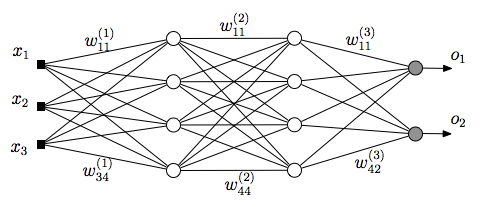
\includegraphics[scale=0.5]{img/MLP}
    \caption{Paveikslėlio pavyzdys}
    \label{img:mlp}
\end{figure}


\section{Eksperimentinio palyginimo rezultatai}
% tablesgenerator.com - converts calculators (e.g. excel) tables to LaTeX
\begin{table}[H]\footnotesize
    \centering
    \caption{Lentelės pavyzdys}
    {\begin{tabular}{|l|c|c|} \hline
    Algoritmas & $\bar{x}$ & $\sigma^{2}$ \\
    \hline
    Algoritmas A  & 1.6335    & 0.5584       \\
    Algoritmas B  & 1.7395    & 0.5647       \\
    \hline
    \end{tabular}}
    \label{tab:table example}
\end{table}

\end{document}